\chapter{آليات التفاعل: الخطوات الأولية والتقريبات}\label{ch:b1:elementary-steps}

يتحد أحادي أكسيد النيتروجين، المتكوّن في محركات السيارات وفي البرق، مع
أكسجين الهواء: \ce{2NO + O2 -> 2NO2}. وتبيّن القياسات المخبرية أن
سرعة هذا التفاعل متناسبة مع $[\ce{NO}]^2[\ce{O2}]$ --- وأنه
يصير \emph{أبطأ} حين يُسخَّن الغاز. فاصطدام واحد بين ثلاثة
جزيئات قد يفسّر الواقعة الأولى، لكنه لا يفسّر الثانية أبدًا: فكل
اصطدام يزداد طاقةً مع ارتفاع درجة الحرارة. والتفسير أن
التفاعل ليس حدثًا واحدًا بل سلسلة من أحداث أبسط، هي
آليته. يعرّف هذا الفصل هذه \omterm{def:b1:elementary-steps:elementary-step}{الخطوات الأولية}، \omterm{def:b1:elementary-steps:energy-profile}{ومخطط
الطاقة} الذي تجري عليه، والتقريبات التي تحوّل
الآلية إلى \omterm{def:b1:rate-laws:order}{قانون سرعة}؛ ويُختم بالحفز، فن فتح
مسلك أيسر.

\begin{recall}
وصف الكتاب الأول (الصف الثاني عشر) \omterm{def:b1:elementary-steps:elementary-step}{آلية التفاعل} بأنها سلسلة من الخطوات
تُرسم بأسهم منحنية، تتكوّن فيها وسائط ثم تُستهلك، ووصف
\omterm{def:b1:elementary-steps:catalyst}{الحفاز} بأنه نوع يسرّع التفاعل دون أن يُستهلك.
وقد عُرّفت \omterm{def:b1:rate-laws:order}{قوانين السرعة} والرتب \omterm{thm:b1:rate-laws:arrhenius}{وقانون أرهينيوس} في
\cref{ch:b1:rate-laws}.
\end{recall}

\section{الخطوات الأولية}

\begin{definition}[الخطوة الأولية، الجزيئية، الآلية]\label{def:b1:elementary-steps:elementary-step}
\emph{الخطوة الأولية}\index{خطوة أولية} تفاعل يجري
في حدث جزيئي واحد، كما هو مكتوب، دون أي
وسيط. و\emph{جزيئيتها}\index{جزيئية} هي عدد
الجسيمات التي تتفاعل في ذلك الحدث: 1 (أحادية الجزيئية، تفكك أو
إعادة ترتيب)، و2 (ثنائية الجزيئية، اصطدام)، ونادرًا 3. و\emph{آلية
التفاعل}\index{آلية التفاعل} مجموعة الخطوات الأولية التي
مجموعها التفاعل الإجمالي. والنوع الذي يتكوّن في خطوة ويُستهلك في
خطوة لاحقة، الغائب عن المعادلة الإجمالية، هو \emph{وسيط
التفاعل}\index{وسيط التفاعل}.
\end{definition}

\begin{proposition}[قانون سرعة الخطوة الأولية]\label{prop:b1:elementary-steps:elementary-law}
\omterm{def:b1:elementary-steps:elementary-step}{للخطوة الأولية} رتبة، ورتبها الجزئية تساوي
معاملاتها الستوكيومترية: فالخطوة $\mathrm{A} \to \dots$ سرعتها $v = k[\mathrm{A}]$؛
و$\mathrm{A} + \mathrm{B} \to \dots$ سرعتها $v = k[\mathrm{A}][\mathrm{B}]$؛
و$2\,\mathrm{A} \to \dots$ سرعتها $v = k[\mathrm{A}]^2$. والعكس غير صحيح:
فالتفاعل الذي تساوي رتبه معاملاته ليس بالضرورة أوليًا.
\end{proposition}

\begin{proof}[استدلال]
تحدث الخطوة الثنائية الجزيئية حين يلتقي جزيء \ce{A} جزيئًا \ce{B}؛ وعدد
هذه اللقاءات في وحدة الحجم والزمن متناسب مع عدد
\ce{A} في وحدة الحجم ومع عدد \ce{B}، ومن ثم مع
$[\ce{A}][\ce{B}]$. وتحدث الخطوة الأحادية الجزيئية لكل جزيء باحتمال
ثابت في وحدة الزمن، ومن ثم بسرعة متناسبة مع $[\ce{A}]$.
\end{proof}

\begin{remark}[لماذا نادرًا ما تتجاوز الجزيئية اثنين]\label{rem:b1:elementary-steps:termolecular}
التقاء ثلاثة جسيمات في اللحظة نفسها، ولكل منها الطاقة والتوجه
المناسبان، حدث نادر؛ والتفاعل ذو \omterm{def:b1:rate-laws:order}{الرتبة الكلية} 3 يكاد يكون
دائمًا نتيجة خطوتين ثنائيتي الجزيئية متتاليتين، كما في
مسألة نهاية الأسبوع.
\end{remark}

\section{مخططات الطاقة}

\begin{definition}[إحداثي التفاعل، مخطط الطاقة، الحالة الانتقالية]\label{def:b1:elementary-steps:energy-profile}
تنتقل الذرات على امتداد \omterm{def:b1:elementary-steps:elementary-step}{الخطوة الأولية} من ترتيب
المتفاعلات إلى ترتيب النواتج؛ والمتغير الذي يقيس هذا التقدم
(طول رابطة يزداد، وطول أخرى يتناقص) هو \emph{إحداثي
التفاعل}\index{إحداثي التفاعل}. والتمثيل البياني للطاقة الكامنة
للنظام على امتداده هو \emph{مخطط الطاقة}\index{مخطط الطاقة}.
وقمته هي \emph{الحالة الانتقالية}\index{حالة انتقالية}،
وهي ترتيب للذرات فيه روابط نصف متكوّنة
ونصف مكسورة، لا يدوم أكثر من اهتزاز جزيئي ولا يمكن
عزله. وارتفاع هذه القمة فوق المتفاعلات هو
حاجز الطاقة للخطوة.
\end{definition}

\begin{omfigure}
\begin{tikzpicture}
\begin{axis}[omprofile, name=a,
  width=0.48\linewidth, height=5.4cm, xmin=0, xmax=10, ymin=-68, ymax=95,
  xlabel={إحداثي التفاعل}, ylabel={الطاقة}]
\addplot[omDef, very thick] table[x=x, y=E] {figdata/out/bachelor-1-energy-profiles-one-step.dat};
\draw[dashed, black!40] (axis cs:0,0) -- (axis cs:10,0);
\draw[<->, omThm] (axis cs:5,0) -- (axis cs:5,79);
\node[omThm, anchor=west, font=\small] at (axis cs:5.1,30) {الحاجز};
\draw[<->, omProp] (axis cs:9.9,0) -- (axis cs:9.9,-40);
\node[omProp, anchor=east, font=\small] at (axis cs:9.8,-14) {$\Delta E$};
\node[anchor=south, font=\small] at (axis cs:5,81) {الحالة الانتقالية};
\node[anchor=north west, font=\small] at (axis cs:0.15,-3) {المتفاعلات};
\node[anchor=north, font=\small] at (axis cs:8.6,-42) {النواتج};
\end{axis}
\begin{axis}[omprofile, at={(a.east)}, anchor=west, xshift=1.2cm,
  width=0.48\linewidth, height=5.4cm, xmin=0, xmax=10, ymin=-64, ymax=95,
  xlabel={إحداثي التفاعل}, ylabel={الطاقة}]
\addplot[omDef, very thick] table[x=x, y=E] {figdata/out/bachelor-1-energy-profiles-two-step.dat};
\node[anchor=south, font=\small] at (axis cs:3,71) {\foreignlanguage{arabic}{ح. انتقالية \babelsublr{1}}};
\node[anchor=south, font=\small] at (axis cs:7,56) {\foreignlanguage{arabic}{ح. انتقالية \babelsublr{2}}};
\node[anchor=north, font=\small, align=center] at (axis cs:5,27) {وسيط};
\node[anchor=north west, font=\small] at (axis cs:0.15,-3) {المتفاعلات};
\node[anchor=north east, font=\small] at (axis cs:10,-43) {النواتج};
\end{axis}
\end{tikzpicture}

{\small يسارًا: مخطط \omterm{def:b1:elementary-steps:elementary-step}{خطوة أولية} واحدة، بحاجزها
وتغير طاقة التفاعل. يمينًا: آلية من خطوتين؛ ويقع
الوسيط في تجويف بين حالتين انتقاليتين. والطاقات
توضيحية.}
\end{omfigure}

\begin{proposition}[الحواجز وقانون أرهينيوس]\label{prop:b1:elementary-steps:barrier}
\omterm{def:b1:rate-laws:activation-energy}{طاقة تنشيط} \omterm{def:b1:elementary-steps:elementary-step}{الخطوة الأولية} قريبة من حاجزها:
فلا يبلغ الحالةَ الانتقالية إلا الاصطدامات التي تحمل تلك الطاقة على الأقل.
ومن أجل الاتجاهين المباشر والعكسي لخطوة، $E_{a,+} -
E_{a,-} = \Delta E$، وهي طاقة تفاعل الخطوة.
\end{proposition}

\begin{proof}[استدلال]
تتسلق الخطوة العكسية الحاجز نفسه من الجهة الأخرى: فارتفاعه
مقيسًا من النواتج يزيد على الارتفاع المباشر بمقدار $-\Delta E$.
\end{proof}

\begin{proposition}[مسلّمة هاموند]\label{prop:b1:elementary-steps:hammond}
تشبه \omterm{def:b1:elementary-steps:energy-profile}{الحالة الانتقالية} \omterm{def:b1:elementary-steps:elementary-step}{لخطوة أولية}، بنيةً وطاقةً،
النوعَ الأقرب إليها طاقةً: النواتجَ في
خطوة شديدة الصعود (ماصة للحرارة)، والمتفاعلاتِ في خطوة شديدة
الهبوط (ناشرة للحرارة). وبالتالي، في الخطوة التي تكوّن وسيطًا عالي
الطاقة، كل ما يثبّت الوسيط يخفض أيضًا
الحاجز المؤدي إليه.
\end{proposition}
\admitted

\section{الخطوة المحدِّدة للسرعة والتوازن المسبق}

\begin{definition}[الخطوة المحدِّدة للسرعة]\label{def:b1:elementary-steps:rds}
في سلسلة من الخطوات، \emph{الخطوة المحدِّدة
للسرعة}\index{خطوة محددة للسرعة} خطوة أبطأ بكثير من كل
الخطوات الأخرى؛ فتساوي السرعة الإجمالية سرعتها، وتتكيف الخطوات الأسرع
معها كما تتبع سيارات الطريق أبطأ نقطة فيه.
\end{definition}

\begin{definition}[تقريب التوازن المسبق]\label{def:b1:elementary-steps:pre-equilibrium}
في \emph{تقريب التوازن المسبق}\index{تقريب التوازن المسبق}
يُفترض أن الخطوة العكوسة السريعة التي تسبق \omterm{def:b1:elementary-steps:rds}{الخطوة المحدِّدة
للسرعة} تبقى في \omterm{def:b1:extent-q-and-k:quantitative}{حالة توازن} طوال الوقت: فتخضع تراكيز
أنواعها لثابت توازنها $K_1 = k_1/k_{-1}$.
\end{definition}

\begin{proposition}[قانون السرعة انطلاقًا من توازن مسبق]\label{prop:b1:elementary-steps:pre-equilibrium-law}
من أجل الآلية
\[
  \mathrm{A} + \mathrm{B} \underset{k_{-1}}{\overset{k_1}{\rightleftharpoons}} \mathrm{I}
  \ \text{(سريعة)}, \qquad
  \mathrm{I} + \mathrm{C} \xrightarrow{\ k_2\ } \mathrm{P} \ \text{(بطيئة)},
\]
تكون السرعة $v = k_2K_1[\mathrm{A}][\mathrm{B}][\mathrm{C}]$، ذات \omterm{def:b1:rate-laws:order}{الرتبة
الكلية} 3، والثابت الظاهري $k = k_1k_2/k_{-1}$.
\end{proposition}

\begin{proof}
السرعة هي سرعة الخطوة البطيئة، $v = k_2[\mathrm{I}][\mathrm{C}]$.
والخطوة الأولى تبقى في \omterm{def:b1:extent-q-and-k:quantitative}{حالة توازن}: $k_1[\mathrm{A}][\mathrm{B}] =
k_{-1}[\mathrm{I}]$، فيكون $[\mathrm{I}] = K_1[\mathrm{A}][\mathrm{B}]$.
وبالتعويض نحصل على النتيجة.
\end{proof}

\section{تقريب الحالة المستقرة}

\begin{theorem}[تفاعلات متتالية من الرتبة الأولى]\label{thm:b1:elementary-steps:consecutive}
من أجل $\mathrm{A} \xrightarrow{k_1} \mathrm{B} \xrightarrow{k_2} \mathrm{C}$،
والخطوتان كلتاهما من الرتبة 1، مع $[\mathrm{A}] = a_0$ و$[\mathrm{B}] =
[\mathrm{C}] = 0$ عند $t = 0$ و$k_1 \ne k_2$:
\[
  [\mathrm{A}] = a_0\eu^{-k_1t}, \qquad
  [\mathrm{B}] = \frac{a_0k_1}{k_2 - k_1}\big(\eu^{-k_1t} - \eu^{-k_2t}\big),
  \qquad [\mathrm{C}] = a_0 - [\mathrm{A}] - [\mathrm{B}] .
\]
ويمر الوسيط بقيمة عظمى عند $t_{\max} = \dfrac{\ln(k_2/k_1)}
{k_2 - k_1}$.
\end{theorem}

\begin{proof}
$\dd[\mathrm{A}]/\dd t = -k_1[\mathrm{A}]$ تعطي $[\mathrm{A}]$. ثم
$\dd[\mathrm{B}]/\dd t + k_2[\mathrm{B}] = k_1a_0\eu^{-k_1t}$، وهي معادلة خطية
من الرتبة الأولى: بالضرب في $\eu^{k_2t}$، $\frac{\dd}{\dd t}
\big([\mathrm{B}]\eu^{k_2t}\big) = k_1a_0\eu^{(k_2-k_1)t}$، وتكاملها
من 0، حيث $[\mathrm{B}] = 0$، هو $[\mathrm{B}]\eu^{k_2t} =
\frac{k_1a_0}{k_2-k_1}(\eu^{(k_2-k_1)t} - 1)$. ويعطي انحفاظ المادة
$[\mathrm{C}]$. وتنعدم مشتقة $[\mathrm{B}]$ حين $k_1\eu^{-k_1t}
= k_2\eu^{-k_2t}$، أي عند $t_{\max}$.
\end{proof}

\begin{definition}[تقريب الحالة المستقرة]\label{def:b1:elementary-steps:qssa}
في \emph{تقريب الحالة المستقرة}\index{تقريب الحالة المستقرة}
(أو شبه المستقرة)، يؤخذ تركيز وسيط شديد
التفاعل، يُستهلك أسرع بكثير مما يتكوّن، ثابتًا
وصغيرًا بعد فترة تحريض قصيرة: فسرعة
تكوّنه تساوي سرعة استهلاكه،
$\dd[\mathrm{I}]/\dd t \approx 0$.
\end{definition}

\begin{proposition}[متى تصح الحالة المستقرة]\label{prop:b1:elementary-steps:qssa-justified}
من أجل $\mathrm{A} \to \mathrm{B} \to \mathrm{C}$ مع $k_2 \gg k_1$: بعد
مدة من رتبة $1/k_2$، يكون $[\mathrm{B}] \approx k_1[\mathrm{A}]/k_2$ (وهو
ما يعطيه $\dd[\mathrm{B}]/\dd t = 0$)، ويبقى $[\mathrm{B}]$ صغيرًا، ويتكوّن
الناتج بالسرعة $\dd[\mathrm{C}]/\dd t \approx k_1[\mathrm{A}]$:
فالخطوة الأولى هي المحدِّدة للسرعة.
\end{proposition}

\begin{proof}
من أجل $k_2 \gg k_1$ و$t \gg 1/k_2$، يكون $\eu^{-k_2t}$ مهملًا بجانب
$\eu^{-k_1t}$ و$k_2 - k_1 \approx k_2$، فيكون $[\mathrm{B}] \approx (a_0k_1/k_2)
\eu^{-k_1t} = k_1[\mathrm{A}]/k_2 \ll [\mathrm{A}]$. ومن ثم
$\dd[\mathrm{C}]/\dd t = k_2[\mathrm{B}] \approx k_1[\mathrm{A}]$.
\end{proof}

\begin{omfigure}
\begin{tikzpicture}
\begin{axis}[name=s,
  width=0.48\linewidth, height=5.2cm, xmin=0, xmax=6, ymin=0, ymax=1.05,
  axis x line=bottom, axis y line=left,
  xlabel={\babelsublr{$k_1t$}}, ylabel={\foreignlanguage{arabic}{التركيز$/a_0$}},
  title={$k_2 = 0.5\,k_1$}, title style={font=\small},
  tick label style={font=\small}, label style={font=\small}]
\addplot[omDef, thick] table[x=t, y=a] {figdata/out/bachelor-1-consecutive-reactions-slow.dat};
\addplot[omThm, thick] table[x=t, y=b] {figdata/out/bachelor-1-consecutive-reactions-slow.dat};
\addplot[omMeth, thick] table[x=t, y=c] {figdata/out/bachelor-1-consecutive-reactions-slow.dat};
\node[omDef, font=\small, anchor=west] at (axis cs:0.4,0.75) {A};
\node[omThm, font=\small, anchor=south] at (axis cs:1.39,0.51) {B};
\node[omMeth, font=\small, anchor=west] at (axis cs:4.5,0.75) {C};
\end{axis}
\begin{axis}[at={(s.east)}, anchor=west, xshift=1.2cm,
  width=0.48\linewidth, height=5.2cm, xmin=0, xmax=6, ymin=0, ymax=1.05,
  axis x line=bottom, axis y line=left,
  xlabel={\babelsublr{$k_1t$}}, ylabel={\foreignlanguage{arabic}{التركيز$/a_0$}},
  title={$k_2 = 20\,k_1$}, title style={font=\small},
  tick label style={font=\small}, label style={font=\small}]
\addplot[omDef, thick] table[x=t, y=a] {figdata/out/bachelor-1-consecutive-reactions-fast.dat};
\addplot[omThm, thick] table[x=t, y=b] {figdata/out/bachelor-1-consecutive-reactions-fast.dat};
\addplot[omMeth, thick] table[x=t, y=c] {figdata/out/bachelor-1-consecutive-reactions-fast.dat};
\addplot[black, dashed] table[x=t, y=bss] {figdata/out/bachelor-1-consecutive-reactions-fast.dat};
\node[omDef, font=\small, anchor=west] at (axis cs:1.4,0.32) {A};
\node[omThm, font=\small, anchor=south west] at (axis cs:2,0.22) {\foreignlanguage{arabic}{\babelsublr{B}، والحالة المستقرة متقطعة}};
\node[omMeth, font=\small, anchor=west] at (axis cs:4.5,0.85) {C};
\end{axis}
\end{tikzpicture}

{\small تفاعلات متتالية $\mathrm{A} \to \mathrm{B} \to \mathrm{C}$.
يسارًا: يتراكم الوسيط ويبلغ قمته عند $k_1t = 1.39$. يمينًا:
حين يُستهلك أسرع بعشرين مرة مما يتكوّن، يبقى صغيرًا
ويتبع قيمة الحالة المستقرة $k_1[\mathrm{A}]/k_2$ (الخط المتقطع) بعد
فترة تحريض قصيرة.}
\end{omfigure}

\begin{method}[قانون السرعة انطلاقًا من آلية]\label{met:b1:elementary-steps:rate-law}
لاستنتاج \omterm{def:b1:rate-laws:order}{قانون سرعة} آلية:
\begin{enumerate}
  \item اكتب سرعة كل \omterm{def:b1:elementary-steps:elementary-step}{خطوة أولية} (\cref{prop:b1:elementary-steps:elementary-law})؛
  \item عبّر عن السرعة الإجمالية بأنها \omterm{def:b1:rate-laws:rate}{سرعة تكوّن} ناتج
        (مقسومة على معامله)؛
  \item احذف كل وسيط \omterm{def:b1:elementary-steps:qssa}{بتقريب الحالة المستقرة}
        ($\dd[\mathrm{I}]/\dd t = 0$، وهي معادلة جبرية) أو، إن سبق
        توازنٌ سريع خطوةً بطيئة، بثابته؛
  \item بسّط في الحالات الحدية التي يغلب فيها حد واحد، وقارن
        بالقانون التجريبي.
\end{enumerate}
\end{method}

\begin{example}[تفاعل محفَّز بالحمض]\label{ex:b1:elementary-steps:acid}
من أجل $\mathrm{S} + \ce{H3O+} \rightleftharpoons \mathrm{SH}^+ + \ce{H2O}$ (سريعة،
ثابتها $K_1$) تليها $\mathrm{SH}^+ + \ce{H2O} \to \mathrm{P} + \ce{H3O+}$ (بطيئة،
$k_2$)، تكون السرعة $v = k_2[\mathrm{SH}^+] = k_2K_1[\mathrm{S}][\ce{H3O+}]$:
من الرتبة الأولى بالنسبة إلى الركيزة وبالنسبة إلى الحمض، مع أن الحمض لا يُستهلك.
\end{example}

\section{الحفز والتحكم في الانتقائية}

\begin{definition}[الحفاز، الحفز المتجانس والحفز غير المتجانس]\label{def:b1:elementary-steps:catalyst}
\emph{الحفاز}\index{حفاز} نوع كيميائي يزيد \omterm{def:b1:rate-laws:rate}{سرعة
التفاعل} دون أن يظهر في معادلته الإجمالية: فهو يُستهلك في إحدى
خطوات الآلية ويتجدد في خطوة لاحقة. وفي
\emph{الحفز المتجانس}\index{حفز متجانس} يكون الحفاز
في \omterm{def:b1:extent-q-and-k:system}{طور} المتفاعلات نفسه (أحماض مذابة، ومعقدات فلزية،
وإنزيمات)؛ وفي \emph{الحفز غير المتجانس}\index{حفز غير متجانس}
يكون طورًا منفصلًا، جسمًا صلبًا عادةً يجري على سطحه
التفاعل (البلاتين، والحديد، والزيوليتات).
\end{definition}

\begin{proposition}[ما يغيّره الحفاز]\label{prop:b1:elementary-steps:catalysis}
يقدم \omterm{def:b1:elementary-steps:catalyst}{الحفاز} آلية جديدة حاجزها أدنى. فهو يسرّع
التفاعلين المباشر والعكسي بالنسبة نفسها، ولذلك يترك
ثابت التوازن والحالة النهائية وطاقة التفاعل
دون تغيير.
\end{proposition}

\begin{proof}
من أجل \omterm{def:b1:elementary-steps:elementary-step}{خطوة أولية} في \omterm{def:b1:extent-q-and-k:quantitative}{حالة توازن}، تتساوى السرعتان المباشرة
والعكسية: $k_+[\text{المتفاعلات}] = k_-[\text{النواتج}]$، فيكون $K = k_+/k_-$.
ومن أجل أي آلية في \omterm{def:b1:extent-q-and-k:quantitative}{حالة توازن}، تكون كل خطوة في \omterm{def:b1:extent-q-and-k:quantitative}{حالة توازن} (وإلا
ظل نوع ما يتغير)، و$K$ هو جداء النسب
$k_+/k_-$ للخطوات. والمسلك المحفَّز يبلغ الحالة النهائية نفسها،
بالثابت نفسه: فأيًّا كان العامل الذي يضرب فيه $k_+$، فإنه يضرب $k_-$
في العامل نفسه.
\end{proof}

\begin{omfigure}
\begin{tikzpicture}
\begin{axis}[omprofile,
  width=0.62\linewidth, height=5.6cm, xmin=0, xmax=10, ymin=-45, ymax=115,
  xlabel={إحداثي التفاعل}, ylabel={الطاقة}]
\addplot[black!60, very thick] table[x=x, y=E] {figdata/out/bachelor-1-energy-profiles-uncatalysed.dat};
\addplot[omMeth, very thick] table[x=x, y=E] {figdata/out/bachelor-1-energy-profiles-catalysed.dat};
\node[anchor=south, font=\small] at (axis cs:5,101) {بلا حفاز};
\node[omMeth, anchor=north, font=\small] at (axis cs:3.5,-6) {مع حفاز};
\draw[<->, omProp] (axis cs:10.4,0) -- (axis cs:10.4,-30);
\draw[dashed, black!40] (axis cs:0,0) -- (axis cs:10.6,0);
\node[omProp, anchor=west, font=\small] at (axis cs:10.5,-15) {\foreignlanguage{arabic}{$\Delta E$ لا يتغير}};
\end{axis}
\end{tikzpicture}

{\small يفتح \omterm{def:b1:elementary-steps:catalyst}{الحفاز} مسلكًا ذا حواجز أدنى (بالأخضر)، كثيرًا ما يكون من
عدة خطوات؛ أما البداية والنهاية، ومن ثم طاقة التفاعل
والتوازن، فهي نفسها.}
\end{omfigure}

\begin{omfigure}
\begin{tikzpicture}[font=\small, >={Stealth}]
  \node[draw=omMeth, rounded corners, fill=omMeth!10, minimum width=2.4cm] (c) at (0,1.6) {الحفاز};
  \node[draw=black!50, rounded corners, fill=black!5, minimum width=2.4cm] (i1) at (2.6,0) {\foreignlanguage{arabic}{المعقد \babelsublr{1}}};
  \node[draw=black!50, rounded corners, fill=black!5, minimum width=2.4cm] (i2) at (0,-1.6) {\foreignlanguage{arabic}{المعقد \babelsublr{2}}};
  \node[draw=black!50, rounded corners, fill=black!5, minimum width=2.4cm] (i3) at (-2.6,0) {\foreignlanguage{arabic}{المعقد \babelsublr{3}}};
  \draw[->, thick] (c) to[bend left=20] node[above right] {+ A} (i1);
  \draw[->, thick] (i1) to[bend left=20] node[below right] {+ B} (i2);
  \draw[->, thick] (i2) to[bend left=20] node[below left] {} (i3);
  \draw[->, thick] (i3) to[bend left=20] node[above left] {$-$ P} (c);
\end{tikzpicture}

{\small دورة حفزية: يربط \omterm{def:b1:elementary-steps:catalyst}{الحفاز} المتفاعلين A وB على
التوالي، ويتحرر الناتج P، ويتجدد \omterm{def:b1:elementary-steps:catalyst}{الحفاز} ليبدأ
من جديد. وتُدرس الدورات الحفزية للمعقدات الفلزية في مجلد السنة
الثانية.}
\end{omfigure}

\begin{omfigure}
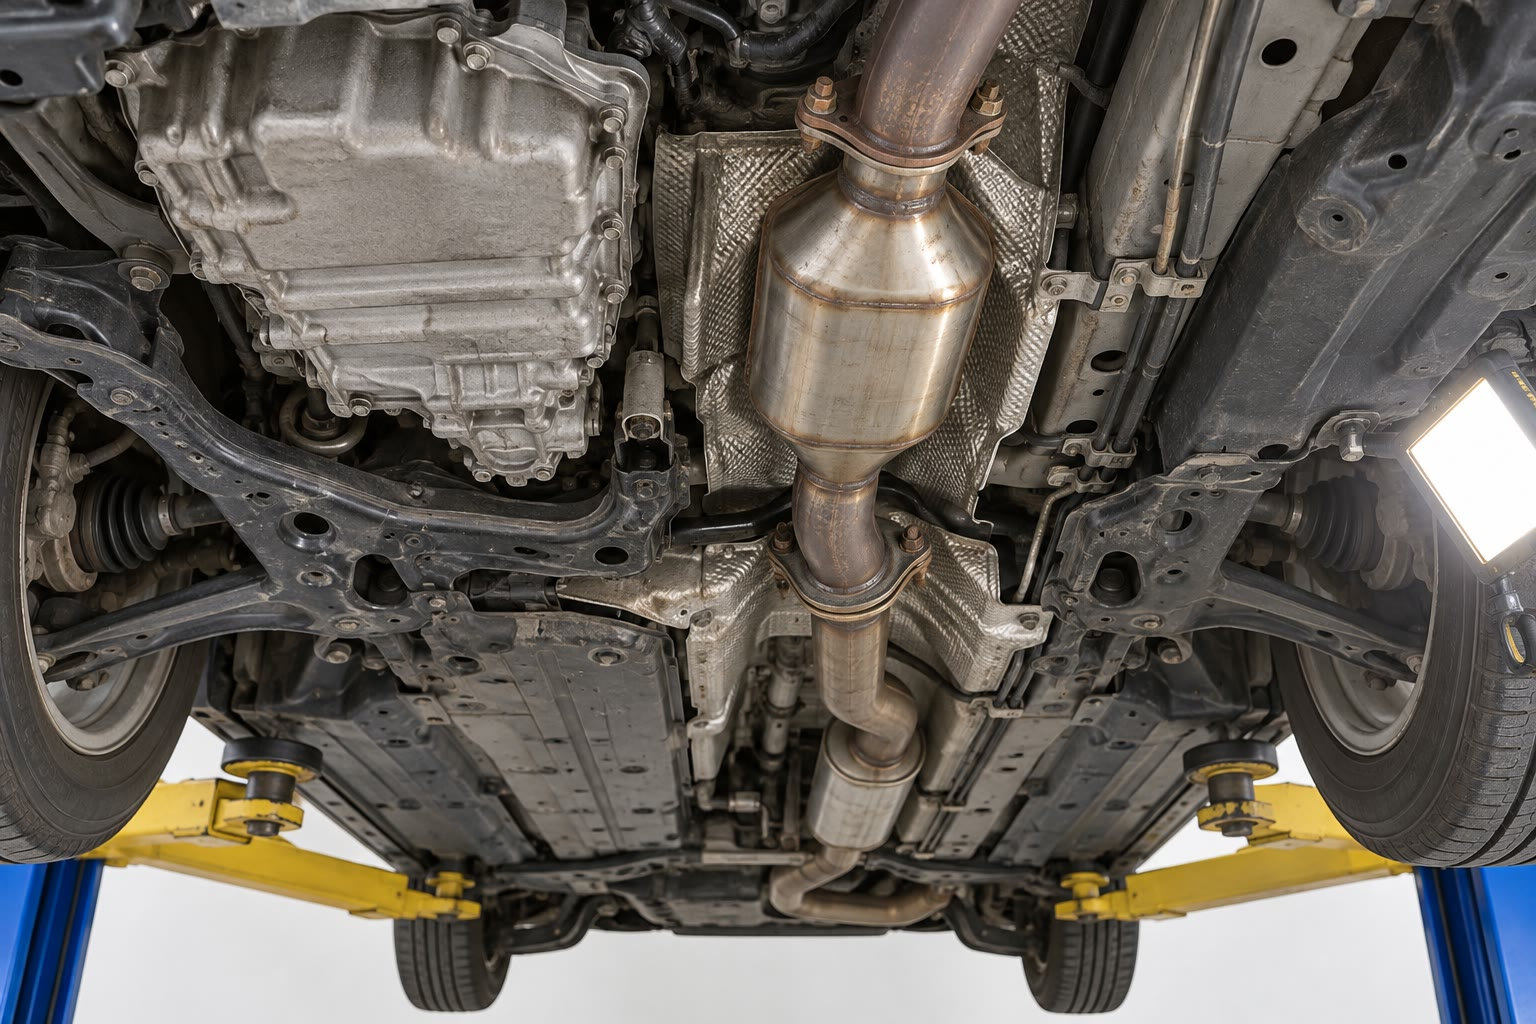
\includegraphics[width=0.5\linewidth]{images/book2/ai/b1-09-catalytic-converter.jpg}

{\small الجهة السفلية لسيارة: الأسطوانة الموجودة في خط العادم
محوِّل حفزي، أي \omterm{def:b1:elementary-steps:catalyst}{حفاز} غير متجانس تتفاعل على سطحه الفلزي
غازات العادم.}
\end{omfigure}

\begin{definition}[التحكم الحركي والتحكم الترموديناميكي]\label{def:b1:elementary-steps:control}
حين يستطيع متفاعل أن يعطي ناتجين عبر مسلكين متنافسين، يكون التفاعل
تحت \emph{تحكم حركي}\index{تحكم حركي} إذا كانت نسب
النواتج محددة بسرعات التكوّن (يغلب الناتج ذو الحاجز
الأدنى)، وتحت \emph{تحكم
ترموديناميكي}\index{تحكم ترموديناميكي} إذا كان المسلكان عكوسين
وبلغ النظام التوازن (يغلب الناتج الأكثر استقرارًا).
\end{definition}

\begin{example}[اختيار الناتج]\label{ex:b1:elementary-steps:control}
يعطي متفاعل الناتج B عبر حاجز قدره \qty{50}{kJ/mol} ($\Delta E =
\qty{-10}{kJ/mol}$) والناتج C عبر حاجز قدره \qty{70}{kJ/mol} ($\Delta E =
\qty{-40}{kJ/mol}$). عند \qty{300}{K} ولأزمنة قصيرة، ومع تساوي
العاملين قبل الأسيين، يتكوّن B أسرع من C بنحو $\exp(20000/(8.314 \times 300)) \approx
3000$ مرة: \omterm{def:b1:elementary-steps:control}{فالتحكم الحركي} يعطي B. أما عند درجة حرارة عالية
ولأزمنة طويلة، فيعود B عبر حاجزه العكسي الصغير، ولا يعود C،
وينتهي النظام إلى C: إنه \omterm{def:b1:elementary-steps:control}{التحكم الترموديناميكي}.
\end{example}

\begin{history}[الحفز، 1835]
جمع الكيميائي السويدي يونس ياكوب برزيليوس سنة 1835 تحت كلمة واحدة
دزينة من الملاحظات المحيّرة --- تحوّل النشا إلى سكر بالأحماض،
وتفكك بيروكسيد الهيدروجين بالفلزات، وأكسدة الكحول على البلاتين ---
وسمّى القوة الخفية العاملة فيها «الحفزية». واحتاج الأمر إلى حركية
أواخر القرن، مع فيلهلم أوستفالد، لتعريف \omterm{def:b1:elementary-steps:catalyst}{الحفاز} بأنه
نوع يغيّر \omterm{def:b1:rate-laws:rate}{سرعة التفاعل} لا توازنه.
\end{history}

\section{تمارين}

\begin{exercise}[$\star$]\label{exo:b1:elementary-steps:1}
أعطِ جزيئية كل خطوة وبيّن أي الخطوات يمكن أن تكون أولية:
(أ) $\ce{N2O5 -> NO2 + NO3}$؛ (ب) $\ce{NO + NO3 -> 2NO2}$؛
(ج) $\ce{2H2 + O2 -> 2H2O}$؛ (د) $\ce{O + O2 + N2 -> O3 + N2}$.
\end{exercise}

\begin{exercise}[$\star$]\label{exo:b1:elementary-steps:2}
اكتب \omterm{def:b1:rate-laws:order}{قانون سرعة} \omterm{def:b1:elementary-steps:elementary-step}{الخطوات الأولية} $\mathrm{A} + \mathrm{B} \to
\mathrm{C}$ و$2\,\mathrm{A} \to \mathrm{B}$ و$\mathrm{A} \to \mathrm{B} +
\mathrm{C}$. ولماذا لا يمكن كتابة \omterm{def:b1:rate-laws:order}{قانون سرعة} تفاعل إجمالي انطلاقًا من
معادلته؟
\end{exercise}

\begin{exercise}[$\star$]\label{exo:b1:elementary-steps:3}
على \omterm{def:b1:elementary-steps:energy-profile}{مخطط الطاقة} ذي الخطوتين المرسوم في هذا الفصل (الوسيط عند
30، والحالتان الانتقاليتان عند 70 و55، والنواتج عند $-40$، بالوحدة
\unit{kJ/mol} فوق المتفاعلات)، عيّن الوسيط
والحالتين الانتقاليتين \omterm{def:b1:elementary-steps:rds}{والخطوة المحدِّدة للسرعة}. هل الخطوة الأولى ماصة للحرارة أم ناشرة لها؟
\end{exercise}

\begin{exercise}[$\star$]\label{exo:b1:elementary-steps:4}
يضرب \omterm{def:b1:elementary-steps:catalyst}{حفاز} \omterm{def:b1:rate-laws:order}{ثابت السرعة} المباشر \omterm{def:b1:elementary-steps:elementary-step}{لخطوة أولية} في
$10^4$. ففي كم يضرب \omterm{def:b1:rate-laws:order}{ثابت السرعة} العكسي؟ وثابت
التوازن؟ والمدة اللازمة لبلوغ التوازن؟
\end{exercise}

\begin{exercise}[$\star\star$]\label{exo:b1:elementary-steps:5}
من أجل $\mathrm{A} \to \mathrm{B} \to \mathrm{C}$ مع $k_1 =
\qty{0.10}{s^{-1}}$ و$k_2 = \qty{0.30}{s^{-1}}$، احسب $t_{\max}$
وأكبر تركيز للنوع $\mathrm{B}$، بوحدة $a_0$.
\end{exercise}

\begin{exercise}[$\star\star$]\label{exo:b1:elementary-steps:6}
من أجل $\mathrm{A} \underset{k_{-1}}{\overset{k_1}{\rightleftharpoons}}
\mathrm{I} \xrightarrow{k_2} \mathrm{P}$، وكل الخطوات من الرتبة 1، طبّق
\omterm{def:b1:elementary-steps:qssa}{تقريب الحالة المستقرة} على $\mathrm{I}$ وبيّن أن $v =
\frac{k_1k_2}{k_{-1} + k_2}[\mathrm{A}]$. ناقش الحالتين $k_2 \gg
k_{-1}$ و$k_2 \ll k_{-1}$.
\end{exercise}

\begin{exercise}[$\star\star$]\label{exo:b1:elementary-steps:7}
تحفّز أيونات اليوديد تفكك بيروكسيد الهيدروجين:
\ce{H2O2 + I- -> H2O + IO-} (بطيئة)، ثم \ce{H2O2 + IO- -> H2O + O2 + I-}
(سريعة). اكتب المعادلة الإجمالية، وعيّن \omterm{def:b1:elementary-steps:catalyst}{الحفاز}
والوسيط، وأعطِ \omterm{def:b1:rate-laws:order}{قانون السرعة}.
\end{exercise}

\begin{exercise}[$\star\star$]\label{exo:b1:elementary-steps:8}
تكوّن خطوة كربوكاتيونًا من جزيء متعادل، وهي عملية
شديدة الصعود. فسّر، مستعينًا بمسلّمة هاموند، لماذا يسرّع المتبادِلُ الذي
يثبّت الكربوكاتيون الخطوةَ أيضًا.
\end{exercise}

\begin{exercise}[$\star\star$]\label{exo:b1:elementary-steps:9}
في \cref{ex:b1:elementary-steps:control}، احسب نسبة ثابتي \omterm{def:b1:rate-laws:rate}{سرعة
تكوّن} B وC عند \qty{300}{K} وعند \qty{600}{K}.
علّق.
\end{exercise}

\begin{exercise}[$\star\star\star$]\label{exo:b1:elementary-steps:10}
يتفكك غاز $\mathrm{A}$ بعد أن يُنشَّط بالاصطدام بأي
جزيء $\mathrm{M}$: $\mathrm{A} + \mathrm{M} \rightleftharpoons
\mathrm{A}^* + \mathrm{M}$ ($k_1$، $k_{-1}$)، ثم $\mathrm{A}^* \to
\mathrm{P}$ ($k_2$). مستعملًا \omterm{def:b1:elementary-steps:qssa}{تقريب الحالة المستقرة} للنوع
$\mathrm{A}^*$، أوجد $v$، وبيّن أن التفاعل من الرتبة 1 تحت ضغط
عالٍ ومن الرتبة 2 تحت ضغط منخفض.
\end{exercise}

\begin{exercise}[$\star\star\star$]\label{exo:b1:elementary-steps:11}
برهن على صيغة $[\mathrm{B}](t)$ في
\cref{thm:b1:elementary-steps:consecutive} وعالج الحالة الخاصة
$k_1 = k_2 = k$، التي فيها $[\mathrm{B}] = a_0kt\,\eu^{-kt}$.
\end{exercise}

\begin{exercise}[$\star\star\star$]\label{exo:b1:elementary-steps:12}
للتفاعل الإجمالي $\mathrm{A} + 2\,\mathrm{B} \to \mathrm{P} +
\mathrm{C}$ \omterm{def:b1:rate-laws:order}{قانون السرعة} التجريبي $v =
k[\mathrm{A}][\mathrm{B}]^2/[\mathrm{C}]$. اقترح آلية فيها توازن مسبق
سريع تفسّره.
\end{exercise}

\section{مسألة: لماذا يتأكسد أحادي أكسيد النيتروجين أسرع في البرد}

\begin{problem}[{مسألة نهاية الأسبوع --- أكسدة أحادي أكسيد النيتروجين ذات الرتبة الثالثة،
وتوازن مسبق عبر المثنوي \ce{N2O2}، ومعالجة الحالة
المستقرة، \omterm{def:b1:rate-laws:activation-energy}{وطاقة تنشيط} ظاهرية سالبة}]
\label{pb:b1:elementary-steps:1}
من أجل \ce{2NO(g) + O2(g) -> 2NO2(g)}، تعطي قياسات السرعات الابتدائية عند
\qty{300}{K} (السرعات بالوحدة \unit{mol.L^{-1}.s^{-1}}):
\begin{center}
\begin{tabular}{cccc}
\hline
التجربة & $[\ce{NO}]_0$ (mol/L) & $[\ce{O2}]_0$ (mol/L) & $v_0$ \\
\hline
1 & \num{1.0e-3} & \num{1.0e-3} & \num{1.0e-5} \\
2 & \num{2.0e-3} & \num{1.0e-3} & \num{4.0e-5} \\
3 & \num{1.0e-3} & \num{2.0e-3} & \num{2.0e-5} \\
\hline
\end{tabular}
\end{center}
\omterm{def:b1:rate-laws:order}{وثابت السرعة} المعيَّن عند \qty{400}{K} أصغر بعشر مرات منه عند
\qty{300}{K}. خذ $R = \qty{8.314}{J/(mol.K)}$.
والآلية المقترحة هي
\[
  \ce{2NO <=> N2O2} \ \ (k_1, k_{-1}, \text{سريعة}), \qquad
  \ce{N2O2 + O2 -> 2NO2} \ \ (k_2, \text{بطيئة}).
\]

\medskip
\noindent\textbf{الجزء الأول --- القانون المرصود.}
\begin{enumerate}
  \item أوجد الرتبتين الجزئيتين بالنسبة إلى \ce{NO} و\ce{O2}.
  \item اكتب \omterm{def:b1:rate-laws:order}{قانون السرعة} واحسب $k$ عند \qty{300}{K}، مع وحدته.
  \item هل يمكن أن يكون التفاعل خطوة واحدة ثلاثية الجزيئية؟ قدّم حجة.
  \item احسب \omterm{def:b1:rate-laws:activation-energy}{طاقة التنشيط} الظاهرية من درجتي الحرارة.
  \item لماذا تستحيل \omterm{def:b1:rate-laws:activation-energy}{طاقة تنشيط} سالبة في \omterm{def:b1:elementary-steps:elementary-step}{خطوة
        أولية}؟
  \item اكتب سرعتي اختفاء \ce{NO} و\ce{O2} بدلالة
        $v$.
\end{enumerate}

\medskip
\noindent\textbf{الجزء الثاني --- التوازن المسبق.}
\begin{enumerate}[resume]
  \item تحقق من أن مجموع الخطوتين هو التفاعل الإجمالي. وسمِّ
        الوسيط.
  \item أعطِ جزيئية كل خطوة.
  \item اكتب سرعة الخطوة البطيئة.
  \item عبّر عن $[\ce{N2O2}]$ \omterm{def:b1:elementary-steps:pre-equilibrium}{بتقريب التوازن المسبق}.
  \item استنتج \omterm{def:b1:rate-laws:order}{قانون السرعة} وقارنه بالتجربة.
  \item عبّر عن الثابت المرصود بدلالة $k_1$ و$k_{-1}$ و$k_2$.
\end{enumerate}

\medskip
\noindent\textbf{الجزء الثالث --- الحالة المستقرة.}
\begin{enumerate}[resume]
  \item اكتب $\dd[\ce{N2O2}]/\dd t$ للآلية كاملة.
  \item طبّق \omterm{def:b1:elementary-steps:qssa}{تقريب الحالة المستقرة} وعبّر عن $[\ce{N2O2}]$.
  \item استنتج \omterm{def:b1:rate-laws:order}{قانون السرعة} $v = \dfrac{k_1k_2[\ce{NO}]^2[\ce{O2}]}{k_{-1} +
        k_2[\ce{O2}]}$.
  \item في أي حالة حدية يؤول إلى نتيجة الجزء الثاني؟
  \item ماذا تصير الرتب في الحالة الحدية المعاكسة؟
  \item أي الحالتين الحديتين تدعمها قياسات الجزء الأول؟
\end{enumerate}

\medskip
\noindent\textbf{الجزء الرابع --- \omterm{def:b1:rate-laws:activation-energy}{طاقة التنشيط} الظاهرية.}
تتبع كل خطوة \omterm{thm:b1:rate-laws:arrhenius}{قانون أرهينيوس}، \omterm{def:b1:rate-laws:activation-energy}{بطاقات التنشيط} $E_1 =
\qty{2}{kJ/mol}$ و$E_{-1} = \qty{40}{kJ/mol}$ و$E_2 =
\qty{15}{kJ/mol}$.
\begin{enumerate}[resume]
  \item اكتب $\ln k$ بدلالة لوغاريتمات $k_1$ و$k_{-1}$
        و$k_2$.
  \item استنتج أن $E_a = E_1 - E_{-1} + E_2$.
  \item فسّر: لماذا يمكن أن يكون لتركيب من \omterm{def:b1:elementary-steps:elementary-step}{الخطوات الأولية} \omterm{def:b1:rate-laws:activation-energy}{طاقة
        تنشيط} ظاهرية سالبة؟
  \item ارسم \omterm{def:b1:elementary-steps:energy-profile}{مخطط الطاقة} إجمالًا: أين تقع \omterm{def:b1:elementary-steps:energy-profile}{الحالة الانتقالية} الثانية،
        بالنسبة إلى المتفاعلات \ce{2NO + O2}؟
  \item بأي عامل تتغير السرعة بين 300 و\qty{400}{K}
        بهذه القيمة؟
  \item احسب \omterm{def:b1:rate-laws:activation-energy}{طاقة التنشيط} الظاهرية من قيم الخطوات،
        وقارنها بنتيجة الجزء الأول.
\end{enumerate}
\end{problem}
